

\section{Design and Implement of Malware IR System}

두 페이즈의 구조도는 Figure 과 같다. 두 페이즈에서 공통으로 존재하는 모듈은 Feature Extractor와 Neural Embedder 가 있다. 벡터 학습 페이즈에는 Classifier 가, 리트리벌 페이즈에는 랭킹 모듈이 포함되어있다. 
% Figure
\begin{figure}
  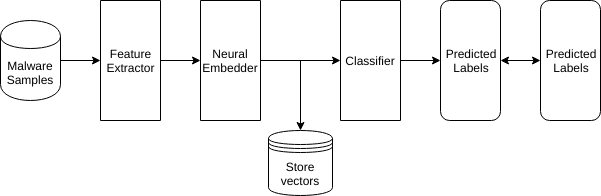
\includegraphics[width=\linewidth]{../figures/train_phase.png}
  \caption{train phase}
  \label{fig:one}
\end{figure}
% Figure
\begin{figure}
  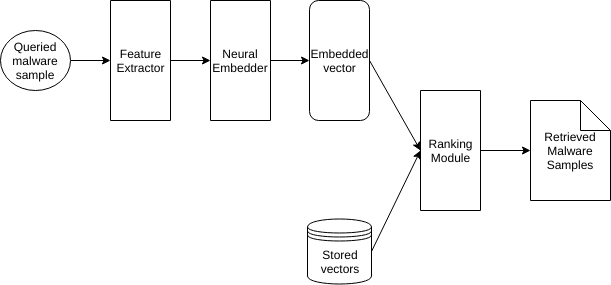
\includegraphics[width=\linewidth]{../figures/retrieval_phase.png}
  \caption{retrieval phase}
  \label{fig:two}
\end{figure}


\subsection{Feature Extractor}

Feature extractor 는 Malware Rawdata 로부터 Handcrafted feature 를 추출하는 모듈이다. Handcrafted feature로 PE 같은경우에는 Size 와 Entropy, Histogram of API Calls, … 등을[*] 추출한다. APK 같은 경우에는 추가적으로 Permission,  … 등의 피쳐를 추출한다. 


\subsection{Neural Embedder}
Neural embedder 는 Feature extractor 모듈에서 추출된 멀웨어의 피쳐들로부터 Representation vector 를 뽑는 모듈이다. theta 로 Parameterized 되어있는 뉴럴 네트워크이며, 파라미터는 벡터 학습 페이즈에서 Auxiliary Task 를 수행하면서 Optimize 된다. 그리고 리트리벌 페이즈에서 파라미터는 freeze 되어 업데이트되지 않는다. 
Neural Embeder 의 네트워크 구조는 Deep and wide 를 사용하였다. Thumbnail 을 받아서 CNN 5 층을 통과시킨 벡터와 나머지 feature 들을 받아서 fully 2 층을 통과시킨 벡터를 concatenate 하고, fully 2 층을 추가로 쌓은 구조를 사용한다. 이렇게 함으로써 우리가 얻을 수 있는 효과는 feature 의 성격에 따라 다른 네트워크 구조로 임베딩 피쳐벡터를 추출함으로써 더 나은 generalization 성능을 얻을 수 있다는 것이다. thumbnail 피쳐는 [malimg 논문 인용] 악성 코드영역 혹은 악성코드를 특징짓는 영역의 로컬리 시프트 인베리언트한 특성을 담기 위해 CNN 을 사용해서 임베딩 피쳐벡터를 추출한다. 


\subsection{Classifier}
% Figure
\begin{figure}
  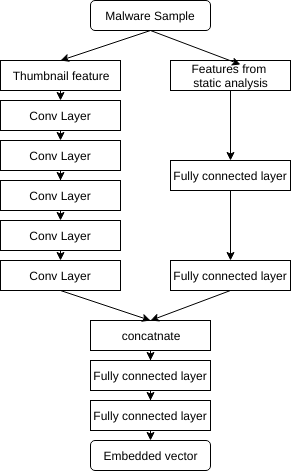
\includegraphics[height=10cm]{../figures/neural_embedder.png}
  \caption{neural embedder}
  \label{fig:three}
\end{figure}

Classifier 모듈은 Neural embedder 를 통과해서 나온 embedding vector 를 받아서 각 레이블 별 확률을 출력해준다. 1차원 fully connected 로 파라미터라이즈드 되어있으며 태스크에 따라 softmax 혹은 sigmoid Activation을 사용하였다. Neural Embeder 모듈과 마찬가지로 벡터 학습 페이즈에서 back propagation 에 의해 파라미터들이 학습되고, 리트리벌 페이즈에서는 프리즈된다. 


\subsection{Ranking Module}
학습 페이즈에 저장해두었던 학습 셋의 임베딩 벡터들과 추출된 벡터의 거리를 재서 k 개의 nearest neighborhood 를 가까운 순서대로 정렬하고 뱉어낸다.


